\chapter{实验分析}
\label{cha:analyze}

\section{跳数}

\subsection{传统路由的情况}

由于在传统路由中,路由条数是完全确定的,
且由于这里使用的图是无向图,因而路由是完全对称的。
这样一来我们只需要分析$u_1$到$u_3$的路径和$u_5$到$u_6$的路径,
即可确定跳数。

经过对图的分析,知路径和跳数如下:

% \usepackage{booktabs}
% \usepackage{caption}

\begin{table}[h]
  \centering
  \begin{tabular}{ccc}
    \toprule
    & 跳数 & 路径 \\
    \midrule
    $ u_1 - u_3 $ & 3 & $ u_1 \rightarrow s_1 \rightarrow s_2 \rightarrow s_3 \rightarrow u_3 $ \\
    $ u_5 - u_6 $ & 3 & $ u_1 \rightarrow s_5 \rightarrow s_4 \rightarrow s_3 \rightarrow u_6 $ \\
    \bottomrule
  \end{tabular}
  \caption{传统路由情况下的条数路径表}
\end{table}

\subsection{SDN路由的情况}

在SDN路由中,我们更改了TCP和UDP的路由。故此处要分析四种路径:

% \usepackage{booktabs}
% \usepackage{caption}

\begin{table}[h]
  \centering
  \begin{tabular}{ccc}
    \toprule
    & 跳数 & 路径 \\
    \midrule
    $ u_1 - u_3(\texttt{TCP}) $ & 3 & $ u_1 \rightarrow s_1 \rightarrow s_2 \rightarrow s_3 \rightarrow u_3 $ \\
    $ u_1 - u_3(\texttt{UDP}) $ & 4 & $ u_1 \rightarrow s_1 \rightarrow s_6 \rightarrow s_4 \rightarrow s_3 \rightarrow u_3 $ \\
    $ u_5 - u_6(\texttt{TCP}) $ & 4 & $ u_1 \rightarrow s_5 \rightarrow s_6 \rightarrow s_2 \rightarrow s_3 \rightarrow u_6 $ \\
    $ u_5 - u_6(\texttt{UDP}) $ & 3 & $ u_1 \rightarrow s_5 \rightarrow s_4 \rightarrow s_3 \rightarrow u_6 $ \\
    \bottomrule
  \end{tabular}
  \caption{传统路由情况下的条数路径表}
\end{table}

\subsection{对比}

从上面的两个表格可以很清楚地看到,使用SDN反而会使得某些情况下的条数变多。
但是从另外的角度上来说,如果不使用SDN,那么实际上只使用了一部分线路,没有充分利用线路资源。

\section{带宽}

\subsection{总体情况}

由于Mininet是网络模拟器而非真实网络,故此处的带宽是我们自定义的带宽。
实际上,这个带宽仅对TCP流量有效,对UDP流量完全没有效果。我们曾经用$1Gbps$
(前面已经叙述过,链路带宽上限为$75Mbps$)的UDP流量进行测试,
结果仍为能够全速传输,且用Wireshark抓包分析后确实产生了相当的流量。
故对于UDP流量的带宽分析是没有意义的。

另外一个问题是,这里有发送带宽和接收带宽,以何者为准呢?理论上应以接收带宽为准,
然而首先发送带宽和接受带宽差别并不大,其次iperf3只能实时测得发送带宽,
故这里以发送带宽为准。

\subsection{传统路由的情况}

在传统路由时,我们同时让$u1$和$u2$进行UDP和TCP测试,带宽-时间图为图3-1和图3-2。

当然,为了证明我们对于UDP流量的分析所言不虚,图3-3展示了UDP流量的带宽-时间图。

从图中可以看到,TCP流量测试持续时间为20秒,UDP流量测试持续时间为10秒。
它们同时进行,这样一来在前10秒内TCP流量被UDP挤占,基本不传输内容。
在后10秒内,带宽在$8-14Mbps$左右波动,进行正常传输。

\begin{figure}[h]
	\centering
	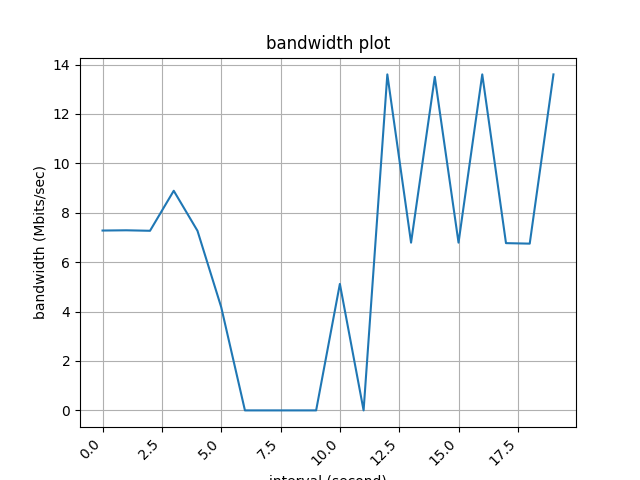
\includegraphics[width=0.8\textwidth]{image/u1.tcp.png}
	\caption{$u_1$进行tcp流量测试带宽-时间图}
 	\label{fig:topo3}
\end{figure}

\begin{figure}[h]
	\centering
	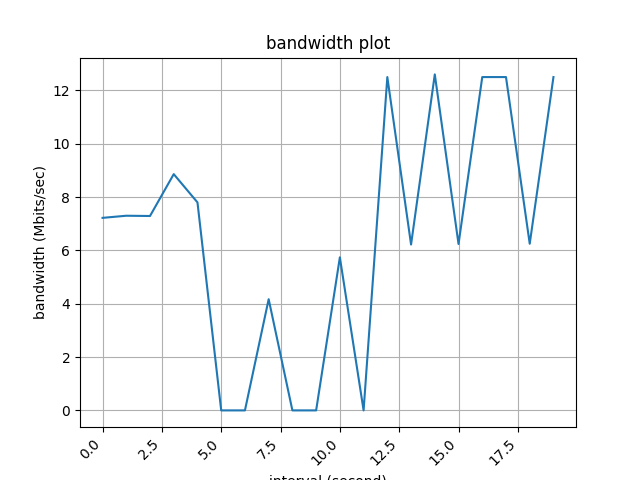
\includegraphics[width=0.8\textwidth]{image/u5.tcp.png}
	\caption{$u_5$进行tcp流量测试带宽-时间图}
 	\label{fig:topo3}
\end{figure}

\begin{figure}[h]
	\centering
	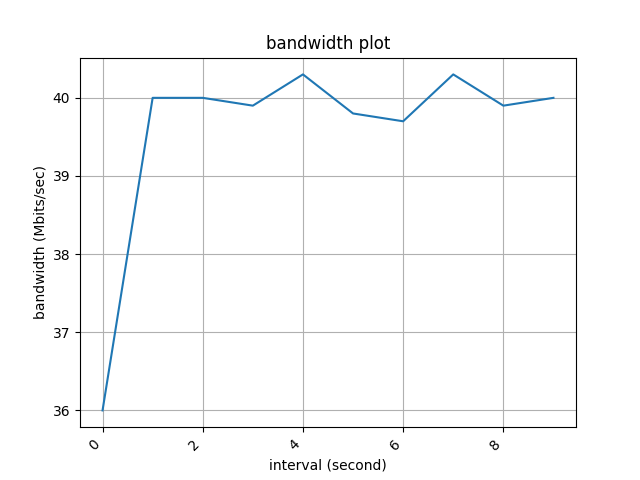
\includegraphics[width=0.8\textwidth]{image/u1.udp.png}
	\caption{$u_1$进行udp流量测试带宽-时间图}
 	\label{fig:topo3}
\end{figure}

平均带宽如下表:

% \usepackage{booktabs}
% \usepackage{caption}

\begin{table}[h]
  \centering
  \begin{tabular}{cc}
    \toprule
    测试 & 带宽 \\
    \midrule
    $ u_1(\texttt{TCP}) $ & 6.44 \\
    $ u_5(\texttt{TCP}) $ & 6.48\\
    \bottomrule
  \end{tabular}
  \caption{传统路由情况下的条数路径表}
\end{table}

\subsection{SDN路由的情况}

在SDN路由时,我们进行了四次测试,分别让UDP发送的带宽为$40Mbps$和$100Mbps$,
这时$u1$、$u5$的TCP带宽-时间图分别为图3-4、图3-5、图3-6和图3-7。

\begin{figure}[h]
	\centering
	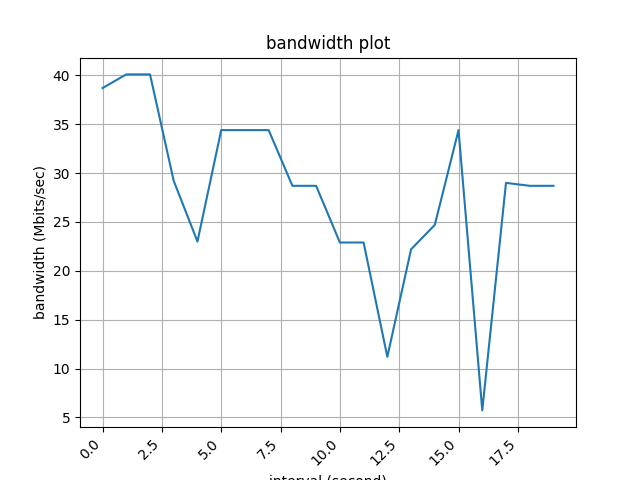
\includegraphics[width=0.8\textwidth]{image/u1-40.tcp.png}
	\caption{$u_1$在udp带宽为$40Mbps$时进行tcp流量测试带宽-时间图}
 	\label{fig:u140}
\end{figure}

\begin{figure}[h]
	\centering
	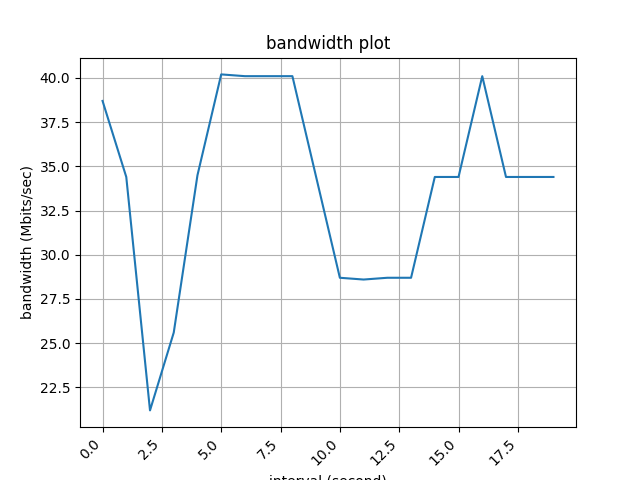
\includegraphics[width=0.8\textwidth]{image/u1-100.tcp.png}
	\caption{$u_1$在udp带宽为$100Mbps$时进行tcp流量测试带宽-时间图}
 	\label{fig:u100}
\end{figure}

\begin{figure}[h]
	\centering
	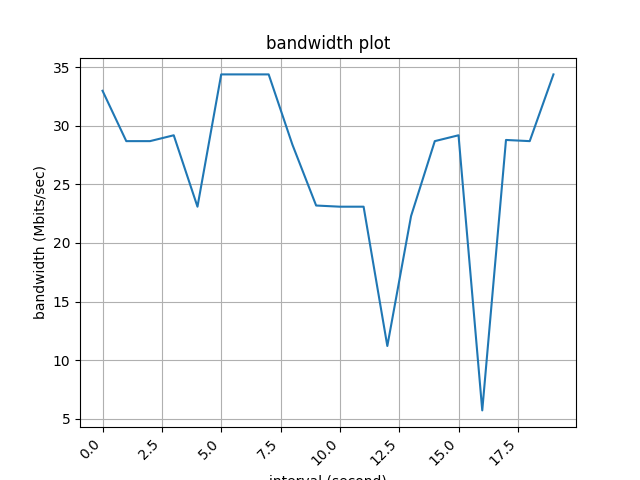
\includegraphics[width=0.8\textwidth]{image/u5-40.tcp.png}
	\caption{$u_5$在udp带宽为$40Mbps$时进行tcp流量测试带宽-时间图}
 	\label{fig:u540}
\end{figure}

\begin{figure}[h]
	\centering
	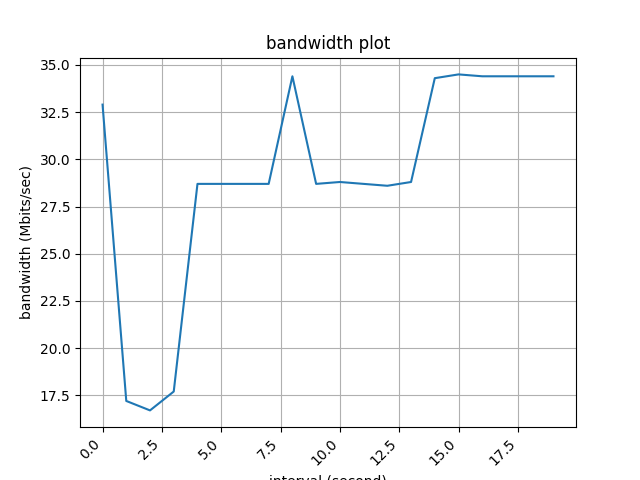
\includegraphics[width=0.8\textwidth]{image/u5-100.tcp.png}
	\caption{$u_5$在udp带宽为$100Mbps$时进行tcp流量测试带宽-时间图}
 	\label{fig:u5100}
\end{figure}

可以看到,虽然带宽有一定波动,但是总体来看还是较为平稳的。

平均带宽如下表:

% \usepackage{booktabs}
% \usepackage{caption}

\begin{table}[h]
  \centering
  \begin{tabular}{cc}
    \toprule
    测试 & 带宽 \\
    \midrule
    $ u_1(\texttt{TCP,UDP=40}) $ & 28.1 \\
    $ u_1(\texttt{TCP,UDP=100}) $ & 33.8 \\
    $ u_5(\texttt{TCP,UDP=40}) $ & 26.6 \\
    $ u_5(\texttt{TCP,UDP=100}) $ & 29.2 \\
    \bottomrule
  \end{tabular}
  \caption{SDN路由情况下的平均带宽表}
\end{table}

\subsection{对比}

从传统路由的实验中,我们可以清楚地看到UDP流量对TCP流量的干扰是非常严重的。
但在SDN路由实验中,由于我们将TCP和UDP进行了分流,这样的干扰不复存在。
这可以从两个方面得到证实:

\begin{enumerate}
  \item 在SDN路由中,增加UDP的带宽,平均带宽没有受到任何影响
  \item 在SDN路由中,平均带宽在前10秒(UDP存在)和后10秒(UDP不存在)没有太大差别。
\end{enumerate}

\section{延迟}

延迟和跳数一样,理论上都是完全确定的。
因为每条路径的延迟是通过Mininet的启动脚本进行设置的,
而Switch的延迟可以忽略不计,故是完全确定的。
然而测试后发现延迟并不是完全确定的,
这可能是由于Switch的延迟不是可忽略的,或Mininet内部有其他机制。

我们进行了两种延迟测试,由于SDN路由时并不对ICMP报文进行特殊处理,
这里只能观察到传统路由下的延迟。

$u1$到$u2$的延迟理论上为$15\ ms$,实际上的延迟测试结果如下:

\begin{figure}[h]
	\centering
	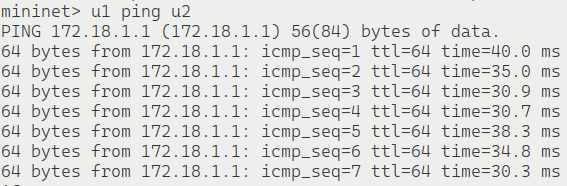
\includegraphics[width=0.8\textwidth]{image/u1pingu2.png}
	\caption{$u1$ ping $u2$的结果}
 	\label{fig:topo3}
\end{figure}

由于ping的时间是往返时间,所以这里的理论值为$30\ ms$. 
可以看到,这和理论值有一定出入。

\section{丢包}

丢包实际上有两种情况:

\begin{itemize}
  \item 线路丢包或由于缓冲区满造成的丢包
  \item 由于TCP的特性,某些包虽然被接受方的网络层接收,但没有被传输层接收
  (比如说序列号在当前接收窗口之前的报文)
\end{itemize}

这两种情况都可以用$\eta$度量,$\eta$的计算公式为:

$$\eta = \frac{D_{recv}}{D_{send}}$$

其中$D_{recv}$是接收方收到的数据,$D_{send}$是发送方发送的数据。

显然地,$\eta$越接近于$1$,丢包率就越低。这里计算出TCP传输时的$\eta$如表3.5.

可见,SDN路由由于对TCP和UDP进行了分流,
能够有效地解决UDP对TCP有干扰造成的丢包问题,提高$\eta$值。

% \usepackage{booktabs}
% \usepackage{caption}
\begin{table}[ht]
  \centering
  \begin{tabular}{ccc}
    \toprule
    测试情况 & 测试对象 & $\eta$ \\
    \midrule
    传统路由,$\texttt{UDP}=40Mbps$ & $u_1 \rightarrow u_3$ & 0.882 \\
    传统路由,$\texttt{UDP}=40Mbps$ & $u_5 \rightarrow u_7$ & 0.903 \\
    SDN路由,$\texttt{UDP}=40Mbps$ & $u_1 \rightarrow u_3$ & 0.997 \\
    SDN路由,$\texttt{UDP}=40Mbps$ & $u_5 \rightarrow u_7$ & 0.987 \\
    SDN路由,$\texttt{UDP}=100Mbps$ & $u_1 \rightarrow u_3$ & 0.991 \\
    SDN路由,$\texttt{UDP}=100Mbps$ & $u_5 \rightarrow u_7$ & 0.991 \\
    \bottomrule
  \end{tabular}
  \caption{$\eta$数值表}
  \end{table}

